\section{Electrical Characterisation of Silicon Sensors}
\label{sec:setup}
\subsection{Setup at CERN}
\label{subsec:setup_principle}
\ref{fig:ALPS_setup} shows a photo of the "Automatic Low Temperature Probe Station" (ALPS) in which the electrical characterisations of the prototype silicon sensors after neutron-irradiation were conducted at CERN. 
A similar setup was created at Texas Tech University.
\begin{figure}[h]
	\centering
	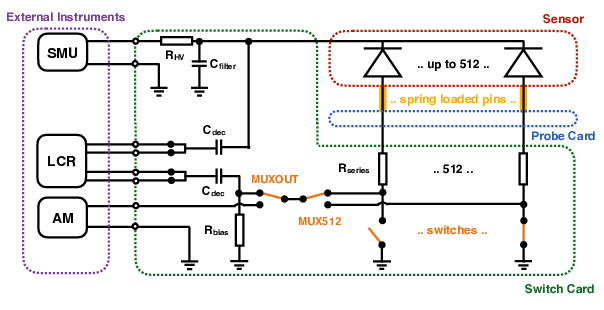
\includegraphics[width=0.75\textwidth]{figures/circuit_cards_updated.png}
	\caption{
		Photo of the Automatic-Low-Temperatre-Probe Staion (ALPS) for the testing of neutron-irradiated CMS HGCAL silicon sensor prototypes at CERN. 
		A similar setup was created at Texas Tech University.
	}
	\label{fig:ALPS_setup}
\end{figure}
Apart from the power supply and meters, all components were installed inside a \textcolor{red}{XXX model} probe station produced by Wentworth Laboratories Ltd.
The sensors were placed on a temperature-controlled chuck and connected to the probe- and switch-card based ARRAY system~\cite{pitters:array2019}.
Through-holes in the cards and the probe station's microscope  enable sufficient sensor-to-pin alignment. 
The high voltage from a Keithley 2410 power supply was provided to the chuck and with it to the sensor's backside.
Two probe cards specific for the high- and for the low-density sensor layouts had been produced and were used in our tests.
Due to the availability of a dedicated pad, also the guard ring could be connected through dedicated pins on these probe cards.
The switch card was operated with a bias resistance (R$_\text{bias}$) of \SI{1}{\mega\ohm} and a high voltage resistance (R$_\text{HV}$) of \SI{12}{\kilo\ohm}.
In this configuration, the ARRAY system is designed to withstand total leakage currents up to $\mathcal{O}(\SI{1}{\milli\ampere})$ and per-pad currents up to \SI{10}{\micro\ampere}.
The voltage drop at R$_\text{HV}$ for the testing of neutron-irradiated sensors is non-negligible and is corrected for in \ref{sec:results}.
The voltage at the silicon pad under test is referred to as "effective bias voltage" in this work.
Per-pad leakage currents were measured with a Keithley \textcolor{red}{6487} whereas total currents were measured directly with the Keithley 2410 power supply.
A Keysight E4980A LCR meter was operated at a frequency (f$_\text{LCR}$) of \SI{2}{\kilo\hertz} for the inference of the per-pad impedance.
This particular frequency was chosen to minimise the error associated to the capacitance~\cite{pitters:array2019}.
It was found empirically the impact on the end capacitance is negligible whereas the derived depletion voltages are increased by about \SI{10}{\percent} when reducing f$_\text{LCR}$ to \SI{500}{\hertz}. 


\subsection{Measurement Procedure}
\label{subsec:setup_procedure}
\begin{itemize}
	\item Measurements conducted at low temperatures to prevent high currents and to protect the system
	\item All measurements were conducted with a chuck temperature of \SI{-40}{\celsius} which was cooled to \SI{-40}{\celsius} during the measurements hereby limiting.
	The probe station itself was flushed with dry air to prevent the formation of ice.
	\item Current compliances to protect system:
	\item Total current compliance: \SI{2}{\milli\ampere}
	\item Per-pad current compliance: \SI{5}{\micro\ampere}
	\item Cells in compliance masked in following leakage current measurements at higher voltages and skipped in subsequent capacitance measurement
	\item 1st round: Per-pad leakage currents (IV), 2nd round: per-pad capacitance
	\item LCR frequency for capacitance measurement is \SI{2}{\kilo\hertz}
	\item Open-correction, serial definition of capacitance
	\item Iterate over all channels at constant voltage, then switch voltage
	\item Total characterisation time: IV = \SI{90}{\minute} (LD)
	\item Total characterisation time: CV = \SI{150}{\minute} (LD)

\end{itemize}